\documentclass[main.tex]{subfiles}
\renewcommand{\thesection}{\Alph{section}}
\begin{document}
\section*{Introduction et rappels}
\subsection*{Types de modulations}
Vu précedemment :
On veux transposer l'information d'un signal $x(t)$ appelé signal modulant
dont le spectre est :
  \begin{center}
  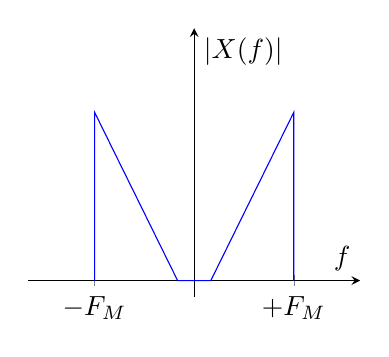
\begin{tikzpicture}
    \begin{axis}%
      [axis lines = middle,
      height = 5cm,
      xlabel = {$f$},
      ylabel = {$|X(f)|$},
      xmin = -5 ,xmax = 5, ymin = -0.1, ymax = 1.5,
      xtick = {-3,3},
      xticklabels = {$-F_M$, $+F_M$},
      ytick=\empty]
      \addplot+[no marks] plot coordinates {(-3,0) (-3,1) (-0.5,0) (0.5,0) (3,1) (3,0)};
    \end{axis}
  \end{tikzpicture}
\end{center}


\begin{defin}
  Signal modulé :
  \[
    s(t) = A(t)\cos(\Phi(t))= A(t)\cos(2\pi f_0 t + \phi(t))
  \]
  où:
  \begin{description}
  \item[A(t)] est l'amplitude instantanée
  \item[$\Phi(t)$]  est la phase instantanée
  \item[$\phi$]  est la déviation de phase par rapport a la porteuse
  \end{description}
\end{defin}

\begin{prop}[Modulation d'amplitude]
  On agit sur l'amplitude de la porteuse.
  \[
    A(t) = k_ax(t)+k_0
  \]
  Avec $k_a$ et $k_0$ des constantes.

\end{prop}
\begin{prop}[Modulation de phase]
  On agit sur la déviation de phase
  \[
    \phi(t) = k_p x(t)+\phi_0
  \]

\end{prop}
\begin{prop}[Modulation de fréquence]
  On agit sur la déviation de fréquence:
  \[
    \Delta f = \frac{1}{2\pi}\deriv[\phi(t)]{t} = k_F x(t)
  \]
\end{prop}

\section{Modulation d'amplitude}
\subsection{Génération d'un signal AM à double bande latérale}
\subsubsection{porteuse supprimée}
\begin{center}
  \begin{circuitikz} \draw
    (0,0) node[mixer,box,anchor=east] (m) {}
    to[amp,box,>,-o] ++(2.5,0) node[right]{$s(t) = kA_0x(t)cos(2\pi f_0 t)$}
    (m.west)  node[inputarrow] {} to[short,-o] ++(-0.8,0) node[left]{$x(t)$}
    (m.east) node[below right]{$k$}
    (m.south) node[inputarrow,rotate=90] {} --
    ++(0,-0.7) node[oscillator,box,anchor=north](osc) {}
    (osc.east) node[right]{$p(t) = A_0\cos{2\pi f_0 t}$};
  \end{circuitikz}
\end{center}

On en déduit le spectre suivant :
  \begin{align*}
    S(f) &= \frac{1}{2}kA_0X(f) * (\delta(f-f_0)+\delta(f-f_0)) \\
         &=\frac{1}{2}kA_0(X(f-f_0)+X(f+f_0))
  \end{align*}
  On peux tracer son spectre :
  \begin{figure}[H]
    \centering
  \begin{tikzpicture}
    \begin{axis}%
      [axis lines = middle,
      height = 5cm,width =15cm,
      xlabel = {$f$},
      ylabel = {$|S(f)|$},
      ytick=\empty,
      xmin = -10 ,xmax = 10, ymin = -0.1, ymax = 1.5,
      xtick = {-9,-6,-3,0, 3,6,9},
      xticklabels = {$-f_0-F_M$,$-f_0$, $-f_0+F_M$,$0$,$f_0-F_M$,$f_0$, $f_0+F_M$,},
      ]
      \addplot+[no marks,color =blue] plot coordinates
      {(-9,0) (-9,1) (-6.5,0) (-5.5,0) (-3,1) (-3,0)};
      \addplot[no marks ,color=blue] plot coordinates
      {(9,0) (9,1) (6.5,0) (5.5,0) (3,1) (3,0)};
    \end{axis}
  \end{tikzpicture}
  \caption{Spectre dans le cadre de la modulation d'amplitude à porteuse supprimée}
  On a un spectre à \emph{double bande latérales} et sans présence explicite de la raie de la porteuse.
\end{figure}

\subsubsection{Modulation d'amplitude à porteuse conservée}
\begin{center}
  \begin{circuitikz} \draw
    (0,0) node[mixer,box,anchor=east] (m) {}  ++(2.5,0) node[mixer,anchor =east] (m2){}
    (m.west)  node[inputarrow] {} to[short,-o] ++(-0.8,0) node[left]{$x(t)$}
    (m.east) node[below right]{$k$}
    (m.east) --  (m2.west) node[inputarrow]{} node[right=-0.2em]{+}
    (m.south) node[inputarrow,rotate=90]{} -- node[midway,left](middle){}
    ++(0,-0.7) node[oscillator,box,anchor=north](osc) {}
    (osc.south) node[below]{$p(t) = A_0\cos{2\pi f_0 t}$}
    (middle) -| (m2.south) node[inputarrow, rotate=90]{} node[above=-0.2em]{+}
    (m2.east) -- ++(1.5,0) node[inputarrow]{}node[right]{$s$};
  \end{circuitikz}
\end{center}
\begin{prop}
Le signal modulé avec porteuse conservée est de la forme:
\[
s(t)  = A_0 (1 + mx(t))\cos(2\pi f_0 t)
\]
\begin{itemize}
\item $e(t) = \frac{x(t)}{max(|x(t)|)}$
\item $m = k.max{|x(t)|}$ est le taux de modulation.
\end{itemize}
\end{prop}
\subsubsection{Sur-,  et sousmodulation}
\begin{figure}[H]
  \centering
  \begin{subfigure}{.5\textwidth}
    \centering
    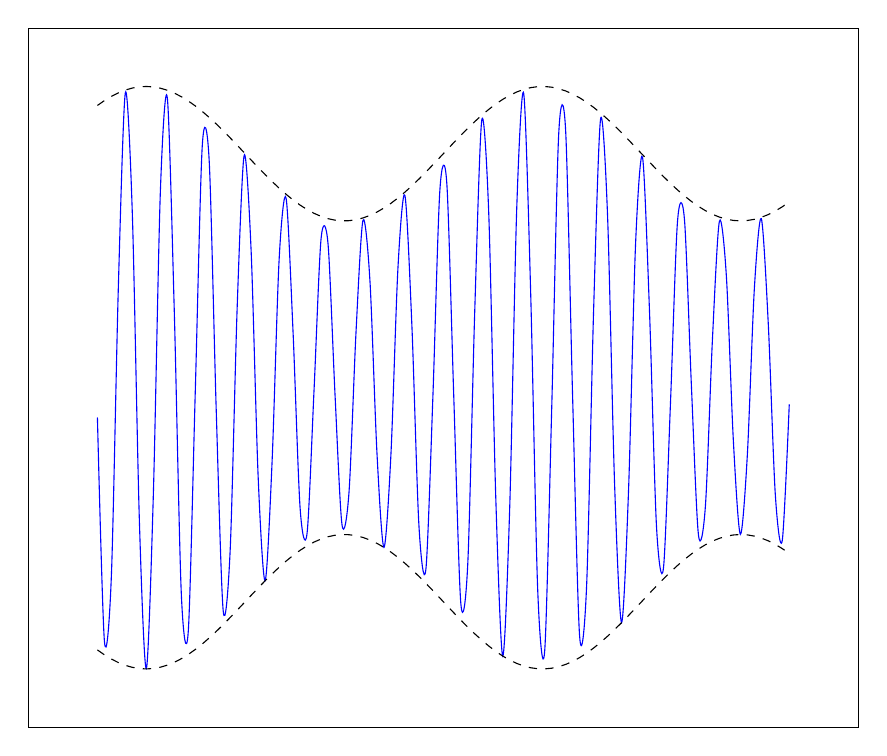
\begin{tikzpicture}
      \begin{axis}
        [samples=100,ticks=none,width=\linewidth,
        domain =-10:10]
        \addplot+[no marks, smooth]{(1+0.3*sin(2*pi*5*x))*cos(2*pi*50*x)};
        \addplot+[no marks, dashed, color = black]{1+0.3*sin(2*pi*5*x)};
        \addplot+[no marks, dashed, color = black]{-1-0.3*sin(2*pi*5*x)};
      \end{axis}
    \end{tikzpicture}
    \subcaption{$m<1$}
  \end{subfigure}%
  \begin{subfigure}{.5\textwidth}
    \centering
    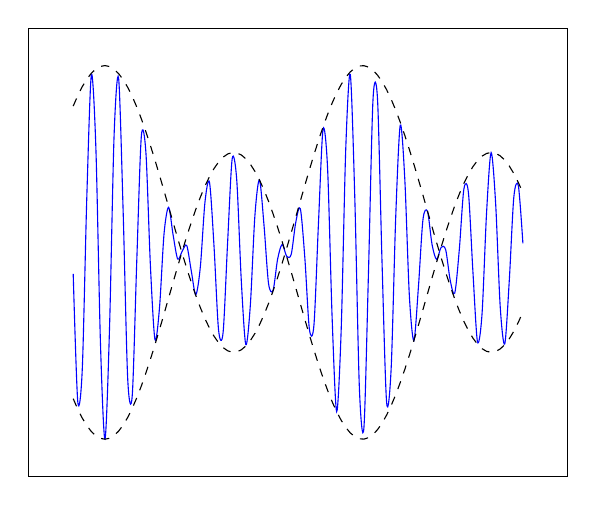
\begin{tikzpicture}
      \begin{axis}
        [samples=100,ticks=none,
        domain =-10:10]
        \addplot+[no marks, smooth]{(1+3.3*sin(2*pi*5*x))*cos(2*pi*50*x)};
        \addplot+[no marks, dashed, color = black]{1+3.3*sin(2*pi*5*x)};
        \addplot+[no marks, dashed, color = black]{-1-3.3*sin(2*pi*5*x)};
      \end{axis}
    \end{tikzpicture}
    \subcaption{$m>1$}
  \end{subfigure}\\
  \begin{subfigure}{.5\textwidth}
    \centering
    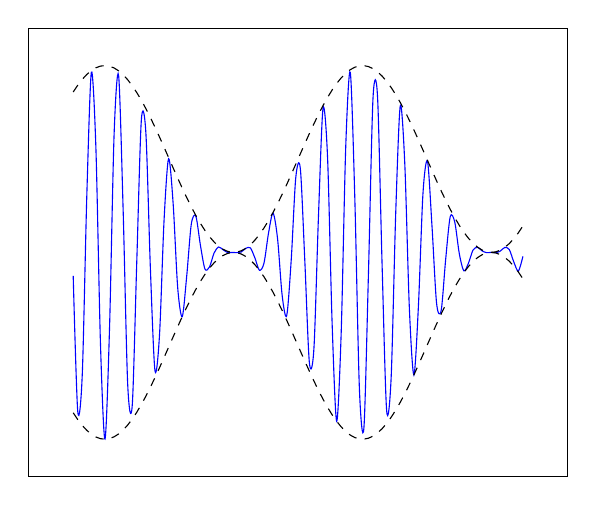
\begin{tikzpicture}
      \begin{axis}
        [samples=100,ticks=none,
        domain =-10:10]
        \addplot+[no marks, smooth]{(1+1*sin(2*pi*5*x))*cos(2*pi*50*x)};
        \addplot+[no marks, dashed, color = black]{1+1*sin(2*pi*5*x)};
        \addplot+[no marks, dashed, color = black]{-1-1*sin(2*pi*5*x)};
      \end{axis}
    \end{tikzpicture}
    \subcaption{$m=1$}
  \end{subfigure}
  \caption{Différentes modulations d'amplitude a porteuse conservée}
\end{figure}

\subsubsection{AM a porteuse conservée, spectre}
Sans surprise :
\begin{figure}[H]
    \centering
  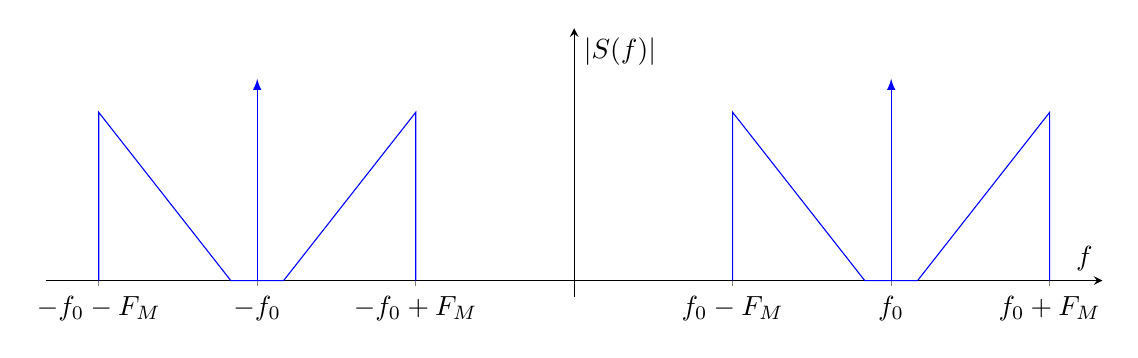
\begin{tikzpicture}
    \begin{axis}%
      [axis lines = middle,
      height = 5cm,width =15cm,
      xlabel = {$f$},
      ylabel = {$|S(f)|$},
      ytick=\empty,
      xmin = -10 ,xmax = 10, ymin = -0.1, ymax = 1.5,
      xtick = {-9,-6,-3,0, 3,6,9},
      xticklabels = {$-f_0-F_M$,$-f_0$, $-f_0+F_M$,$0$,$f_0-F_M$,$f_0$, $f_0+F_M$,},
      ]
      \addplot+[no marks,color =blue] plot coordinates
      {(-9,0) (-9,1) (-6.5,0) (-5.5,0) (-3,1) (-3,0)};
      \addplot[no marks ,color=blue] plot coordinates
      {(9,0) (9,1) (6.5,0) (5.5,0) (3,1) (3,0)};
      \draw[-latex,blue] (axis cs:-6,0) -- (axis cs: -6,1.2);
      \draw[-latex,blue] (axis cs:6,0) -- (axis cs: 6,1.2);
    \end{axis}
  \end{tikzpicture}
  \caption{Spectre dans le cadre de la modulation d'amplitude à porteuse conservée}
\end{figure}

  On retrouve le même encombrement, toujours double bande latérale.

  \begin{prop}
    on défini le rapport entre puissance utile au final et la puissance émise :
    \[
      \rho = \frac{m^2 P_e}{1+m^2P_e}
    \]
  \end{prop}
  \subsection{Démodulation par détection d'enveloppe ou cohérente}

  Système peu couteux , mais nécessite $m < 1 $ :
  \begin{figure}[H]
    \centering
    \begin{circuitikz}
      \draw (0,0) to[open, v=$s(t)$] (0,2) to[D,l=$D_1$] (2,2) to[R,l_=$R_1$] (2,0)
      (2,2) -- (3.5,2) to[C,l_=$C_1$,v^<=$u(t)$] (3.5,0) (0,0) -- (2,0)node[ground]{} -- (3.5,0);
    \end{circuitikz}
    \caption{Circuit détecteur de crête}
  \end{figure}
  \begin{prop}
    Pour obtenir une bonne détection il faut :
    \[
      \frac{1}{2\pi f_0} \ll R_1C_1 < \frac{\sqrt{1-m^2}}{2\pi m F_M}
    \]
\end{prop}
\begin{proof}

\emph{issue de la préparation du TP3}

$D_1$ est une diode Schottky à faible tension de seuil, on la néglige donc dans le modèle de la diode considérée.
\begin{itemize}
\item Lorsque la diode est passante :
  \begin{center}
    \begin{minipage}[r]{0.4\linewidth}
      \begin{circuitikz}
        \draw (0,0) -- (2,0) -- (4,0) to[C,l_=$C_1$,v^<=$r(t)$] (4,-2) -- (0,-2) to[open,v=$s(t)$] (0,0)
        (2,0) to[R,l=$R_1$] (2,-2);
      \end{circuitikz}
    \end{minipage}%
    \begin{minipage}[l]{0.4\linewidth}
      le condensateur se charge et on a
      \[r(t)=s(t)\]
    \end{minipage}
  \end{center}
\item Lorsque la diode est bloquée:
  \begin{center}
    \begin{minipage}[r]{0.4\linewidth}
      \begin{circuitikz}
        \node (A) at (0,0){}; % pas propre
        \draw (2,0) -- (4,0) to[C,l_=$C_1$,v^<=$r(t)$] (4,-2) -- (2,-2)
        (2,0) to[R,l=$R_1$] (2,-2);
      \end{circuitikz}
    \end{minipage}
    \begin{minipage}[l]{0.4\linewidth}
      \begin{align*}
        i_c = -\frac{r(t)}{R_1} &= C_1 \dot{r}(t)\\
        \tau \dot{r}(t) + r(t) &= 0 \quad\text{; avec } \tau= R_1C_1\\
                       r(t) &= r_0e^{-\frac{t-t_0}{\tau}}
      \end{align*}
      Avec $r_0$ valeur en début de la décharge ie $r_0=s(t_1) = S_p(1+m\cos(\Omega t))$.
    \end{minipage}
  \end{center}
\item Dans la phase de décharge : la pente de la droite de décharge est alors :
\[
  \left.\frac{dr(t)}{dt}\right|_{t=t_1} = -\frac{S_p}{R_1C_1}(1+m\cos(\Omega t))
\]
\item la pente de l'enveloppe vaut :
  \[
\left.\frac{ds(t)}{dt}\right|_{t=t_1} = -m\Omega S_p\sin(\Omega t_1)
  \]
  Pour que la restitution soit bonne il faut que la pente de la décharge soit \emph{légèrement} plus faible que la pente de l'enveloppe.
  \begin{align*}
    -\frac{S_p}{R_1C_1}(1+m\cos(\Omega t_1)) &< -m \Omega S_p\sin(\Omega t_1)\\
    R_1C_1 &< \frac{1+m\cos(\Omega t_1)}{m\Omega \sin(\Omega t_1)}
  \end{align*}

  On étudie donc la fonction :
  \[
    y(t) = \frac{1+m\cos(\Omega t)}{m\Omega \sin(\Omega t)}
  \]
  \begin{align*}
    \frac{dy(t)}{dt}= 0 &\iff  \frac{d}{dt}\left(\frac{1}{sin(\Omega t)}+m \frac{1}{tan(\Omega t)}\right) = 0 \\
                        &\iff \frac{\Omega \cos(\Omega t)}{\sin(\Omega t)^2}-m\Omega\frac{1}{\sin(\Omega t)^2} = 0\\
                        &\iff  \Omega t_1 = arccos(-m)
  \end{align*}
  Alors :
  \[
    y(t_1) \leq y(\arccos(-m))=\frac{1-m^2}{\Omega m \sin(\arccos(-m))} = \frac{1-m^2}{\Omega m\sqrt{1-m^2}} = \frac{\sqrt{1-m^2}}{\Omega m}
  \]
  Donc :
  \[
    \boxed{R_1C_1 = \frac{\sqrt{1-m^2}}{2\pi F m}}
  \]

\item La modulation de la sinusoïde est trop forte pour pouvoir etre suivi par le montage détecteur de crète. En effet:
  \[
    R_1C_1 \xrightarrow{m \to 1} 0
  \]

\item
  Lorsque la fréquence du signal modulant se rapproche de la fréquence de la porteuse la détection crête ne fonctionne pas non plus (phénomène de battement).
\end{itemize}
\end{proof}
\subsubsection{Démodulation AM cohérente : principe}
\begin{center}
  \begin{circuitikz} \draw
    (0,0) node[mixer,box,anchor=east] (m) {}
    to[lowpass,box,>,-o] ++(2.5,0) node[right]{$d(t)$}
    (m.west)  node[inputarrow] {} to[short,-o] ++(-0.8,0) node[left]{$s(t)$}
    (m.east) node[below right]{$k$}
    (m.south) node[inputarrow,rotate=90] {} --
    ++(0,-0.7) node[oscillator,box,anchor=north](osc) {}
    (osc.east) node[right]{$p(t) = A_r\cos{2\pi (f_0 +\Delta f) t+\Delta\phi}$};
  \end{circuitikz}
\end{center}
On dispose de la porteuse à la reception (récupérer par VCO ou générée indépendamment).
\[
  u(t)=\frac{kA_rA_0}{2}x(t)(\cos(2\pi \Delta f t +\Delta\phi)+cos(2\pi(2f_0+\Delta f)t+\Delta\phi))
\]
Dans le cas de la porteuse supprimée ( en considérant $\Delta f = 0 $ et $\Delta \phi = 0$):

\begin{figure}[H]
  \centering
  \begin{tikzpicture}
     \begin{axis}%
       [axis lines = middle,
       at = {(0,0)},
      height = 5cm,width =12cm,
      xlabel = {$f$},
      ylabel = {$|S(f)|$},
      ytick=\empty,
      xmin = -25 ,xmax = 25, ymin = -0.1, ymax = 1.5,
      xtick = {-11,11},
      xticklabels = {$-f_0$,$f_0$},
      ]
      \addplot+[no marks,color =blue] plot coordinates
      {(-12,0) (-12,1) (-11,0) (-11,0) (-10,1) (-10,0)};
      \addplot[no marks ,color=blue] plot coordinates
      {(12,0) (12,1) (11,0) (11,0) (10,1) (10,0)};
    \end{axis}
    \begin{axis}%
      [axis lines = middle,
      at = {(0,-5cm)},
      height = 5cm,width =12cm,
      xlabel = {$f$},
      ylabel = {$|U(f)|$},
      ytick=\empty,
      xmin = -25 ,xmax = 25, ymin = -0.1, ymax = 1.5,
      xtick = {-22,22},
      xticklabels = {$-2f_0$,$2f_0$},
      ]
      \addplot+[no marks,color =blue] plot coordinates
      {(-23,0) (-23,1) (-22,0) (-22,0) (-21,1) (-21,0)};
      \addplot[no marks ,color=blue] plot coordinates
      {(23,0) (23,1) (22,0) (22,0) (21,1) (21,0)};
      \addplot[no marks ,color=blue] plot coordinates
      {(1,0) (1,1) (0,0) (0,0) (-1,1) (-1,0)};
      \addplot[no marks, dashed, color=black]  plot coordinates
      {(-2.5,0) (-1,1.2) (1,1.2) (2.5,0)};
      \draw[-latex](axis cs:3,1) node[right] (box){
        \begin{tabular}{c}
          Passe-Bas,\\
          $F_M<f_c\ll2f_0$
        \end{tabular}
} (box) to[bend left] (axis cs:1.75,0.6);
    \end{axis}

    \draw[-latex] (0,1cm) to[bend right] node[midway,left]{Démodulation} (0,-4cm);
  \end{tikzpicture}

\caption{Spectre des signaux considérés}
\end{figure}
En $d(t)$ on retrouve bien $x(t)$ a un facteur multiplicatif pres.  (et une constante additive si porteuse conservée)

\paragraph{Remarque}: si on a pas un synchronisme parfait (phase et fréquence) les spectres se superposent en effet :
\[
  d(t) = \frac{kA_0A_r}{2}x(t)cos(2\pi\Delta f t+\Delta\phi)
\]
\subsection{Modulation AM particulière}
\subsubsection{Modulation d'amplitude en quadrature}
\subsubsection{Modulation à bande latérale unique}
pour réduire le support fréquenciel du signal modulé.
\subsubsection{Modulation à Bande latérale atténuée}

\section{Modulation angulaire : FM et PM}
\subsection{Principe, aspect spectral}

\begin{defin}
   \begin{description}
    \item[Déviation de fréquence]~\\
      $\Delta f(t) = \frac{1}{2\pi}\deriv[\phi(t)]{t}=k_Fx(t)$
    \item[Excursion en fréquence]~\\
      $\Delta f_{max}=\max |k_f x(t)|$
    \end{description}%
      \[
        s_{FM}(t)= A_0 \cos(2\pi f_0t +2\pi k_f \int_0^tx(\tau)d\tau)
      \]
  \end{defin}
\begin{defin}
\begin{description}
    \item[Déviation de phase]~\\
      $\Phi(t) = k_p x(t)+\phi(0)$
    \item[Excursion en phase]~\\
      $\Delta \Phi_{max}=\max |k_f x(t)|$
      \[
        s_{PM}(t)= A_0 \cos(2\pi f_0t +2\pi k_p x(t))
      \]
    \end{description}
\end{defin}


\begin{prop}
  Pour une modulante sinusoïdale $x(t) = A_X \cos(2\pi F_X t)$ on a :
  \[
    s_{FM}(t)=A_0 \cos\left(2\pi f_0 t +\frac{\Delta f_{max}}{F_X}sin(2\pi F_{X}t)\right)
  \]
  Et
  \[
    S_{PM} =A_0 \cos\left(2\pi f_0 t +\Delta \phi_{max}sin(2\pi F_{X}t)\right)
  \]
  On défini \emph{l'indice de modulation} $\beta$ comme :
  \[
    \beta =
    \begin{cases}
      \Delta \phi_{max} & \text{en PM}\\
      \frac{k_FA_X}{F_X} & \text{en FM}
    \end{cases}
  \]
\end{prop}

\subsubsection{Spectre pour une modulante sinusoïdale}

\begin{thm}[identité de Bessel]
  \[
    e^{jx\sin(y)}=\sum_{n=-\infty}^{+\infty}J_n(x)e^{jny}
  \]
  Avec la fonction de bessel de première espèce d'indice $n$:
  \[
    J_n(x)=\frac{1}{\pi} \int_{0}^{\pi}cos(xsin(\theta)-n\theta)d\theta
  \]
  On a de plus $J_{-n}(\beta)= (-1)^nJ_n(\beta)$
\end{thm}

Ainsi on a pour le signal modulé en FM :
\[
  s_{FM} = A_0 \Re(e^{2j\pi f_0t}e^{j\beta\sin(2\pi F_Xt)}) = A_0 \Re \left(e^{2j\pi f_0 t} \sum_{n=-\infty}^{+\infty}J_n(x)e^{j2\pi F_x t}\right)
\]

[Insert Spectre FM]

On a un encombrement en fréquence infini , mais la fonction de bessel est décroissante ainsi :
\begin{prop}[règle de Carson]
  98\% de la Puissance du signal modulé se trouve dans la bande de fréquence utile $B_u$ donnée par :
  \[
    B_u = 2F_X(\beta+1)
  \]
  Cela se généralise pour tout signal $x(t)$ :
  \[
    B_u = 2F_M(\beta_{nom}+1) = 2\Delta f_{max}+2F_M
  \]
\end{prop}

\paragraph{Remarque} Ce n'est qu'un des critère possibles. De manière générale le support fréquentielle en FM est plus large qu'en AM.

Dans le cas d'une phase $\phi(t) \ll \frac{\pi}{2}$ on peux faire un DL et on retrouve un spectre semblabe a celui d'une AM à double bande latérale :

\[
s(t) = A_0 \Re(e^{2j\pi f_0t}e^{j\phi(t)}) \simeq  A_0 \Re(e^{2j\pi f_0t}(1+j\phi(t))) = A_0 \cos(2\pi f_0t) - \phi(t)\sin(2\pi f_0t)
\]

[insert Graphics]

En FM er à DSP de bruit constante on a interet a préaccentuer les aigus et de $x(t)$ par rapport aux graves (apres démodulation désacentuation).


\subsection{Méthode de génération d'une modulation angulaire}
\subsubsection{FM par oscillateur controllé en tension}
\subsubsection{FM par régulation de fréquence porteuse}
\subsubsection{PM par réactance variable}
\subsubsection{Modulation PM à base de PLL}
\subsection{Méthode de démodulation angulaire}
\subsubsection{Démodulatateur a PLL}
\subsubsection{Autre démodulateurs}
\paragraph{Démodulateur par déphasage}
\paragraph{Démodulateur FM par comptage}

\section{Modulation et bruit}
\subsection{Différentes origines du bruit electronique}
Le Bruit est une tension nusibile qui se superposant au signal utile. Les principales sources de bruits sont :
\begin{itemize}
\item bruit thermique
\item bruit electromagnétique
\end{itemize}
Dans la suite on considère que le bruit est \emph{additif} , centrée , ergodique, de puissance finie...
On le note $n(t)$ et $D_n(f)$ sa DSP. (TF de la fonction d'autocorrélation)\footnote{cf. UE 451}.
\subsubsection{Bruit thermique}
Le bruit thermique est issu du mouvement brownien des électrons libre dans un conducteur , proportionnel à la température (agitation thermique)
\begin{center}
  \begin{circuitikz}
    \draw (0,0) to[R,l={R bruyante},v=$v(t)$] (0,2) -- (2,2) to[voltmeter,l=$V_{eff}$] (2,0) -- (0,0);
  \end{circuitikz} $\iff$%
  \begin{circuitikz}
    \draw (0,0) to[V,l=$n$] (0,2) to[R,l={R non bruyante}] (0,4) -- (2,4) to[R,l={R non bruyante},v=$v$] (2,0) -- (0,0);
  \end{circuitikz}
\end{center}
\begin{prop}
  On a alors $v = n/2$ et :
  \[
    <n^2> = 4k_B T R \Delta f = 4k_B T \Re(Z)
  \]
  \[
    D_n = 4k_B T R (en V^2/Hz)
  \]
  La DSP est constante (bruit blanc).
\end{prop}

\subsubsection{Température équivalente}
par analogie avec le bruit thermique on peux définir la température d'un bruit blanc pour d'autr source de bruit. Par exemple le bruit d'une antenne en reception : $T = 300 K$ (vers le sol) , $T=qq K$ (vers le ciel)). On parle alors d'antenne "froide" (peu de pertubation) .

\subsubsection{Autres bruits}
\begin{description}
\item[bruit blanc de grenaille] (Cf Schottky, 1918) : nombre faible de porteur de charge franchissant une barrière de potentiel
\item[bruit de scintillation] DSP en $1/f $ : fluctuation de grandeur physique (densité de défaut chargé, rugosité d'interface..)
\item[Bruit coloré] DSP en $f^n$ (traité par des ampli ,CF TD10).
\end{description}

Tous ces différents bruit s'ajoute pour former un DSP d'allure :


[Insert graphics, plancher de bruit]

\subsection{Bruit dans une chaine de Quadripole}
{\LARGE
\begin{center}
  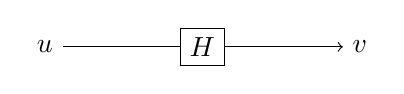
\begin{tikzpicture}
    \node (e) at (0,0) {$u$};
    \node[rectangle,draw] (f) at (2,0) {$H$};
    \node (s) at (4,0) {$v$};
    \draw[->] (e) -- (f) -- (s);
  \end{tikzpicture}
\end{center}}
\begin{defin}
D'après la formule d'interférence:
\[D_v(f) = |H(f)|^2D_u(f)+D_p(f)\]
  On défini le \emph{facteur de bruit} d'un quadripole $Q$ de fonction de transfert $H$:

    \begin{align*}
      F &= \frac{\text{DSP de bruit total en sortie}}{\text{DSP de bruit si Q non bruyant}}\\
        &= \frac{|H(f)|^2D_u(f)+D_p(f)}{|H(f)|^2D_u(f)}\\
        &= 1 + \frac{D_p(f)}{|H(f)|^2D_u(f)} \geq 1
     \end{align*}
   \end{defin}

   On peux également définir la température équivalente de bruit du quadripôle:

   \paragraph{Hypothèse}
   \begin{itemize}
   \item Adaptation d'impédance entre Q et les connections ($Z_c$ supposée réelle)
   \item[$\implies$] Optimisation du transfert de puissance car pas de reflexionsur Q
   \item Bruit Thermique par une impédance $Z_c$ placée en entrée de Q.
   \end{itemize}

   \begin{center}
     \begin{circuitikz}
       \draw (0,0) to[R, l=$Z_c@ T_e$,v=$u$] (0,2) -- (2,2) to[R, l=$Z_c$] (2,0) -- (0,0);
       \draw (1.5,-0.2) rectangle (4,2.2) node[above]{Q};
       \draw (4,2) -- (5,2) to[R] (5,0) --(4,0);
     \end{circuitikz}
   \end{center}

   \begin{prop}
     On a :
     \[\left.
       \begin{array}{r}
         D_u(f) = k_B T_eZ_c \\
         ~\\
         D_p(f  = |H(f)|^2k_BT_QZ_C
       \end{array}\right\} \implies F = 1 + \frac{T_Q}{T_e}
     \]
   \end{prop}

\subsubsection{Quadripole en cascade}
   Pour deux quadripole en série de gain $H_1$ et $H_2$ :

{\LARGE
\begin{center}
  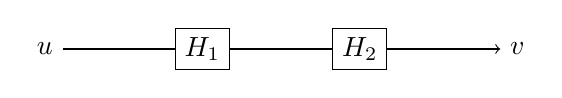
\begin{tikzpicture}
    \node (e) at (0,0) {$u$};
    \node[rectangle,draw] (f1) at (2,0) {$H_1$};
    \node[rectangle,draw] (f2) at (4,0) {$H_2$};
    \node (s) at (6,0) {$v$};
    \draw[->] (e) -- (f1) -- (f2) -- (s);
  \end{tikzpicture}
\end{center}}


\begin{thm}[Formule de Friis]
  Pour la mise en cascade de deux quadripoles le facteur de bruit total est:
  \[
    F_{tot} = F_1 + \frac{1}{|H_1(f)|^2}(F_2-1)
  \]
  La formule se généralise par récurrence pour $N$ quadripoles en série:
  \[
    F_{tot} = F_1 + \frac{1}{|H_1(f)|^2}(F_2-1) + \frac{1}{|H_1(f)|^2|H_2(f)|^2}(F_3-1)+ \dots + \frac{1}{|H_1(f)|^2|H_2(f)|^2|H_{N-1}(f)|^2}(F_N-1)
  \]
\end{thm}
\paragraph{Remarque}
On a tout intêret à placer un amplificateur faible bruit (LNA\footnote{Low Noise Amplifier}) pour minimiser le facteur de bruit total (cf TD11).

\subsubsection{Facteur de bruit et RSB}
{\Large
\begin{center}
  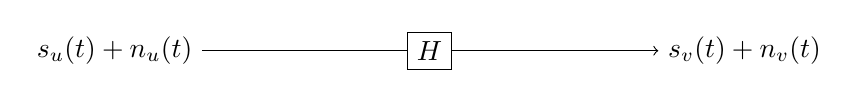
\begin{tikzpicture}
    \node (e) at (0,0) {$s_u(t)+n_u(t)$};
    \node[rectangle,draw] (f) at (4,0) {$H$};
    \node (s) at (8,0) {$s_v(t)+n_v(t)$};
    \draw[->] (e) -- (f) -- (s);
  \end{tikzpicture}
\end{center}}
\begin{prop}
  Dans le cas où $|H(f)|$ et les DSP \emph{sont indépendantes de $f$ dans la bande de fréquence} B considérée, alors :
   \[
     F = \frac{D_{n_v}}{|H|^2D_{n_u}} = \frac{S_{ueff^2}}{S_{veff^2}}\frac{D_{nv}}{D_{nu}} = \frac{(S/N)_{entree}}{(S/N)_{sortie}}
   \]
\end{prop}
\subsection{Efficacité vis-à-vis du bruit en démodulation [WIP]}
\subsubsection{Contexte}
\begin{center}
  \begin{circuitikz}
\draw (0,0) to[tline] ++(2,0) to[twoport,t={\tiny capteur}] ++(2,0)to[twoport,t={\tiny preamp}] ++(2,0) to[amp] ++(2,0) to[twoport, t={\tiny Demod},-o]++(2,0) node[right]{$\alpha x(t)+n_s(t)$};
  \end{circuitikz}
\end{center}
Modélisation du bruit (décomposition analytique transformée de hilbert)
\[
n_e  = \Re(n_I(t)+jn_Q(t)exp(2j2\pi f_0 t))
\]
But: calculer :
\[
  \eta =\frac{<\alpha^2x^2>/<n_s^2>}{<c^2><n_e^2>}
\]
\subsubsection{Cas de l'AM}
\[
  \eta = \frac{<n_e^2>}{(1/2)kA_1<x^2>} = 2
\]
efficacité faible mais garantie
\paragraph{Autre Modulation AM}
\begin{description}
\item[BLU]  $\eta =1$
\item[BL atténuée]  $\eta = \frac{2}{1+c^2}$ avec $0\le c \le 1$
\item[Quadrature] $\eta =2$
\item[DB+porteuse] $\eta= 2 \frac{2k^2<x^2>}{1+k^2<x^2>}$
\end{description}

\subsubsection{Démodulation angulaire}
\paragraph{généralité}

\paragraph{Démodulation PM}
\[
  \eta = 2 k_P^2 <x^2> \simeq 2\beta^2
\]
Peux devenir $\gg 1 $ mais il faut RSB grand et $B_u$ large.

\paragraph{Démodulationn FM}
\[
  \eta = 6 \frac{k_f^2<x^2>}{F_M^2} \simeq 6 \beta^2
\]


\end{document}
